\documentclass[10pt,a4paper,titlepage]{article}
\usepackage[utf8]{inputenc}
\usepackage{amsmath}
\usepackage{amsfonts}
\usepackage{amssymb}
\usepackage{amsthm}
\usepackage{biblatex}
\usepackage{mathtools}
\usepackage[bottom]{footmisc}
\usepackage{pgfplots}
\usepackage[hypertexnames=false]{hyperref}
%\usepackage{parskip}
\pgfplotsset{compat=1.16}

\usetikzlibrary{patterns}

\addbibresource{references.bib}
%\bibliography{references}

\author{Felix Fritz}
\title{The Bondareva-Shapley Theorem}

\theoremstyle{plain}
\newtheorem{thm}{Theorem}[section] % reset theorem numbering for each chapter

\theoremstyle{definition}
\newtheorem{definition}[thm]{Definition} % definition numbers are dependent on theorem numbers
\newtheorem{example}[thm]{Example} % same for example numbers
\newtheorem{corollary}[thm]{Corollary}

\begin{document}

\maketitle

\tableofcontents
\pagebreak

\section{Cooperative Games and the Core}
Before diving into the concept of balanced collections, balanced games and the Bondareva-Shapley Theorem, I want to establish a basic understanding of cooperative games, imputations and the core, mainly as it is described in Robert P. Gilles book \cite{gilles}, pp. 12--13, 18--20 and 29--35.

\begin{definition}
    The pair $(N, v)$ is a \textit{cooperative game} if $N$ is a finite player set and $v: 2^N \rightarrow \mathbb{R}$ is a characteristic function that assigns to every coalition $S \subseteq N$ an attainable payoff $v(S)$ such that $v(\emptyset) = 0$.
    
    For every player set $N$ we denote by $\mathcal{G}^N$ the class of all characteristic functions on $N$.
\end{definition}
Simply put, in a cooperative game collective payoff values are defined for every possible coalition between players. A coalition with no players leads to a payoff of zero.

Suppose for a given cooperative game all players form a grand coalition generating a total payoff of $v(N)$. The ways in which this collective wealth can be distributed is described by a vector $x \in \mathbb{R}^N$, each element $x_i$ indicating what player $i \in N$ would receive.
If this vector fulfills the requirement needed for efficiency and individual rationality, then it is described as an \textit{imputation}.

\begin{definition}
    An \textit{imputation} in the cooperative game $v \in \mathcal{G}^N$ is a vector $x = (x_1, ..., x_n) \in \mathbb{R}^N$ satisfying
    \[
        \begin{aligned}
            &x(N) = v(N) && \quad \text{(Efficiency)}\footnotemark\\
            &x_i \geq v(i)\text{ for every player } i \in N && \quad \text{(Individual rationality)\footnotemark}
        \end{aligned}
    \]
    \footnotetext[1]{For a given vector $x \in \mathbb{R}^N$ and a coalition $S \subseteq N$, $x(S)$ refers to the sum of elements $x_i$ for each player $i \in S$: $x(S) = \sum_{i \in S}x_i$}
    \footnotetext{Formally we would need curly braces around $i$ in the payoff function $v$ $\rightarrow v(\{i\})$. Because it is obvious that $v(i)$ indicates the payoff for a coalition containing the single player $i$, I will omit the braces.}
    The set of all vectors satisfying the efficiency and individual rationality constraint is the \textit{imputation set}.
    \begin{equation}\label{eq:imputation}
        I(N, v) \coloneqq \{x \in \mathbb{R}^N \mid x(N) = v(N),\quad x_i \geq v(i) \quad \forall i \in N\}
    \end{equation}
\end{definition}

With the imputation set, each player is ensured to receive his individual value at minimum.

If each possible coalition $S \subseteq N$ is taken into account to verify that the value from an imputation $x(S) = \sum_{i \in S}x_i \geq v(S)$, then the imputation is \textit{coalitionally rational}.

\begin{definition}\label{def:core}
    A collection of coalitionally rational imputations is the \textit{core} of a cooperative game.
    \begin{equation}\label{eq:core}
        \mathcal{C}(N, v) \coloneqq \{x \in I(N, v) \mid x(S) \geq v(S)\quad \forall S \subseteq N\}
    \end{equation}
\end{definition}


%%% CHAPTER 2 - Bondareva-Shapley Theorem %%%


\pagebreak
\section{Bondareva-Shapley Theorem}
In the following chapter I will discuss the properties of cooperative games with a nonempty core and introduce the notion of balancedness, which leads me to the Bondareva-Shapley Theorem.

\subsection{Nonempty Cores}
This section's focus will be on some of the properties that need to apply for a cooperative game to have at least one imputation that is coalitionally rational, or in other words has a nonempty core.

\begin{example}
    A cooperative game with $N = 2$ players has the following attainable payoffs: $v(\emptyset) = 0, v(1) = v(2) = 2, v(1, 2) = 3$.

    Determining if a core exists in such a situation may be trivial to solve, but with only two players this gives us the opportunity to plot a graph and visualize the solution concept.
    
    Because this is only a two-player game, there are no coalitions other than the grand coalition. This means that every imputation is automatically inside the core.
    
    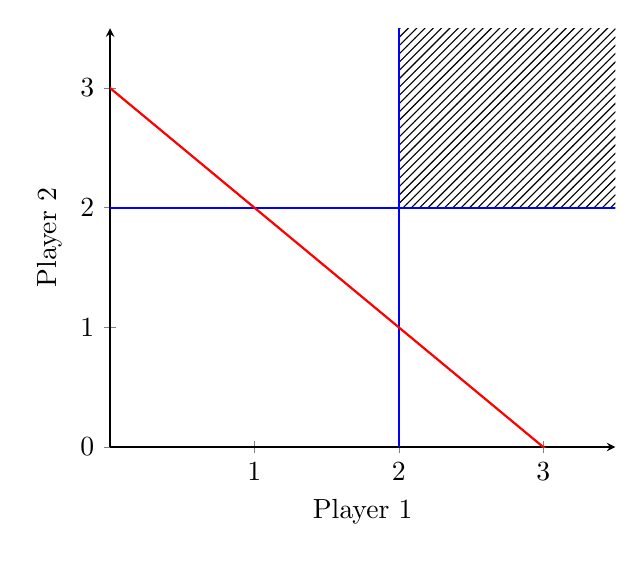
\begin{tikzpicture}
        
        \begin{axis}[no marks,
            axis lines = left,
            xlabel = {Player 1},
            ylabel = {Player 2},
            xmin = 0, xmax = 3.5,
            ymin = 0, ymax = 3.5,
            xtick={1,2,3},
            width=8cm
        ]
            
            %what player 1 wants
            \filldraw [draw=none,pattern=north east lines] (2, 2) rectangle (3.5, 3.5);
            \addplot [blue, thick]{2};
            \addplot [blue, thick] coordinates {(2,0)(2,3.5)};
            

            %efficient payoff function
            \addplot [color=red, thick]{-x+3};
        \end{axis}
        % \filldraw [draw=none,pattern=north east lines] (3.6, 3) rectangle (6.5, 5.5);
            
    \end{tikzpicture}
\end{example}

Because the grand coalition generates a value of 3, an efficient vector $x(N) = x_1 + x_2 = 3$. From this we can derive the function $f(x_2) = 3 - x_1$, which is shown in the graph by the red diagonal line.

The horizontal and vertical lines could be described as the "individually rational" plots, indicating that because of $v(1) = v(2) = 2$ each player in a coalition would like to receive a payoff of 2 at minimum. This means that the smallest attained payoff that would cause the players to form a grand coalition is at the point where the two lines intersect, which is at $(2, 2)$ generating a payoff of 4. From this point, every vector to the upper right would be seen as profitable by the players.

Because none of the actual vectors on $f(x_2)$ cross that region, the cooperative game has an empty core. For a game with two players to have a nonempty core, $v(1, 2) \geq v(1) + v(2)$ must hold, which would be at $v(1, 2) \geq v(1) + v(2) = 2 + 2 = 4$ in the example's case.

Let's further investigate what properties have to apply for a three-player game to have a nonempty core.

\begin{example}\label{ex:findvalue}
    We are given a cooperative game with $N = 3$ players generating the following payoffs:

    \begin{tabular}{c | c c c c c c c}
        $S$ & $\emptyset$ & $\{1\}$ & $\{2\}$ & $\{3\}$ & $\{1, 2\}$ & $\{1, 3\}$ & $\{2, 3\}$\\
        \hline
        $v(S)$ & 0 & 2 & 2 & 1 & 3 & 4 & 6
    \end{tabular}

    What would the minimum payoff $v(1, 2, 3)$ have to be for the players to form a grand coalition?\vspace{10pt}

    To start off, consider the imputation set. For this it is only necessary to find a vector $x \in \mathbb{R}^3$ all vectors that fulfill $x_i \geq v(i)$.

    If every element of $x$ is set equal to the payoff of $v(i)$, this gives us a vector $x = (2, 2, 1)$. From this we derive that a payoff of $5$ would be sufficient for the game to have a nonempty imputation set.

    Clearly this is not the answer however, because players 2 and 3 would much rather get together than cooperate in a grand coalition. Thus, let's consider putting those two together and letting player 1 work on his own. This generates a collective value of $v(1) + v(2, 3) = 8$.

    To verify if this is correct, an imputation $x$ must be found so it is efficient ($x(N) = 8$) and individually and coalitionally rational. For now, I will choose $x = (2, 3, 3)$. This results in the following equations:

    \begin{alignat*}{7}
    x_1 &+ &x_2 &+ &x_3 &= 8 \quad&=&\quad 8 = v(1, 2, 3)\\
    x_1 &+ &x_2 &  &    &= 5 &\geq &\quad 3 = v(1, 2)\\
    x_1 &  &    &+ &x_3 &= 5 &\geq &\quad 4 = v(1, 3)\\
        &  &x_2 &+ &x_3 &= 6 &\geq &\quad 6 = v(2, 3)\\
    x_1 &  &    &  &    &= 2 &\geq &\quad 2 = v(1)\\
        &  &x_2 &  &    &= 3 &\geq &\quad 2 = v(2)\\
        &  &    &  &x_3 &= 3 &\geq &\quad 1 = v(3)
    \end{alignat*}

    This shows that a payoff of 8 would be enough for all three players to form a grand coalition.
\end{example}

However, looking for an arbitrary imputation that \textit{might} be in the core set may not always be as trivial as it was for our example, especially if such problems should be solved computationally. Furthermore finding a payoff vector should be irrelevant if we're only interested in the total attained payoff.

To find a \textit{"value-based"} approach, I will make use of M. Maschler, E. Solan and S. Zamir's book "Game Theory" \cite{maschler} on page 691 ff.

Because the payoff vector is efficient ($x(N) = v(N)$), the inequalities from example \ref{ex:findvalue} can be transformed as followed.

\begin{align}
    v(1) + v(2) + v(3) &\quad\leq\quad v(1, 2, 3)\\
    v(1, 2) + v(3) &\quad\leq\quad v(1, 2, 3)\\
    v(1, 3) + v(2) &\quad\leq\quad v(1, 2, 3)\\
    v(2, 3) + v(1) &\quad\leq\quad v(1, 2, 3)
\end{align}

This can be extended to a final inequality.

\begin{align*}
    (x_1+x_2)+(x_1+x_3)+(x_2+x_3) &\quad \geq \quad v(1, 2) + v(1, 3) + v(2, 3)\\[6pt]
    2*(x_1+x_2+x_3) &\quad \geq \quad v(1, 2) + v(1, 3) + v(2, 3)\\
    v(1, 2, 3) &\quad \geq \quad \frac{1}{2} v(1, 2) + \frac{1}{2} v(1, 3) + \frac{1}{2} v(2, 3)
\end{align*}

\addtocounter{thm}{-1}
\begin{example}\label{ex:valuebased}
    \textit{(continued)}

    Substituting the inequalities from previously where a vector $x$ was chosen with the inequalities just introduced, we get:
    \begin{align*}
        v(1, 2, 3) = 8\quad & \geq \quad 5 = v(1) + v(2) + v(3)\\
        v(1, 2, 3) = 8\quad & \geq \quad 4 = v(1, 2) + v(3)\\
        v(1, 2, 3) = 8\quad & \geq \quad 6 = v(1, 3) + v(2)\\
        v(1, 2, 3) = 8\quad & \geq \quad 8 = v(2, 3) + v(1)\\
        v(1, 2, 3) = 8\quad & \geq \quad 6.5 = 0.5*v(1, 2) + 0.5*v(1, 3) + 0.5*v(2, 3)
    \end{align*}
\end{example}

Those five inequalities are in fact already enough to prove that a payoff of 8 would make a grand coalition feasible. The reason for this will be discussed in more detail later on.



%%%% SUBSECTION 2.2 BALANCED COLLECTIONS %%%%

\subsection{Balanced Collections and Balancing Coefficients}
Each inequality in example \ref{ex:valuebased} \textit{(continued)} looks at the collective wealth of a \textit{balanced collection} of coalitions, each collection with its own set of \textit{balancing coefficients}. M. Maschler\cite{maschler} sums it up with the following table.\vspace{8pt}

\begin{tabular}{ | r l | c | }
    \multicolumn{2}{c}{Collection of coalitions} & \multicolumn{1}{c}{Coefficients}\\[2pt]
    \hline & & \\[-8pt]
    $\mathcal{B}_1 =$ & $\{\{1\}, \{2\}, \{3\}\}$ & $(1, 1, 1)$\\[2pt]
    $\mathcal{B}_2 =$ & $\{\{1, 2\}, \{3\}\}$ & $(1, 1)$\\[2pt]
    $\mathcal{B}_3 =$ & $\{\{1, 3\}, \{2\}\}$ & $(1, 1)$\\[2pt]
    $\mathcal{B}_4 =$ & $\{\{2, 3\}, \{1\}\}$ & $(1, 1)$\\[2pt]
    $\mathcal{B}_5 =$ & $\{\{1, 2\}, \{1, 3\}, \{2, 3\}\}$ & $(\frac{1}{2}, \frac{1}{2}, \frac{1}{2})$\\[2pt]
    \hline
\end{tabular}\vspace{8pt}

$\mathcal{B}_1$ through $\mathcal{B}_4$ are partitions of $N = \{1, 2, 3\}$ with each player appearing exactly once. This always gives us a set of coefficients where each element is 1. From this a "partition" rule can be deducted.

\begin{corollary}
    Let a cooperative game with $N$ players have a nonempty core. A partition is a collection of coalitions $\mathcal{B} = \{S_1, S_2, ..., S_k\}$ satisfying $S_i, S_j \subsetneq N, S_i \cap S_j = \emptyset$ iff\footnote{iff is shorthand for "if and only if", also represented with the math symbol $\Leftrightarrow$} $i \neq j, S_1 \cup S_2 \cup ... \cup S_k = N$.

    Then for every partition $\mathcal{B}$ it must be the case that

    \begin{align}
        v(N) \geq \sum_{S \in \mathcal{B}} v(S)
    \end{align}
\end{corollary}

The goal now is to find a property that also includes the non-partition $\mathcal{B}_5$ from our three-player example. To do this I will use Maschler's\cite{maschler} definition of Index Matrices on page 693.

\begin{definition}
    Let $\mathcal{B} = \{S_1, S_2, ..., S_k\}$ be a collection of nonempty coalitions. The incidence matrix $\mathcal{M}$ of $\mathcal{B}$ is the incidence matrix with k rows (one for each coalition) and n columns (one for each player) with each index $x_{ij}$ at column $i = {0, ..., n}$ and row $j = {0, ..., k}$ defined as follows:

    \begin{equation*}
        x_{ij} =
        \begin{cases}
            1, & \text{if}\ i \in S_j\\
            0, & \text{otherwise}
        \end{cases}
    \end{equation*}
\end{definition}

To give some examples, an incidence matrices for the collections $\mathcal{B}_1 = \{\{1\}, \{2\}, \{3\}\}$, $\mathcal{B}_2 = \{\{1, 2\}, \{3\}\}$ and $\mathcal{B}_5 = \{\{1, 2\}, \{1, 3\}, \{2, 3\}\}$ would look like this.\vspace{8pt}

$
\bordermatrix{
\mathcal{M}_1 & 1 & 2 & 3 \cr
S_1 & 1 & 0 & 0 \cr
S_2 & 0 & 1 & 0 \cr
S_3 & 0 & 0 & 1 \cr
}
$\hspace{50pt}$
\bordermatrix{
\mathcal{M}_2 & 1 & 2 & 3 \cr
S_1 & 1 & 1 & 0 \cr
S_2 & 0 & 0 & 1 \cr
}
$\hspace{50pt}$
\bordermatrix{
\mathcal{M}_5 & 1 & 2 & 3 \cr
S_1 & 1 & 1 & 0 \cr
S_2 & 1 & 0 & 1 \cr
S_3 & 0 & 1 & 1 \cr
}
$\vspace{8pt}

Interestingly enough, if we take each matrix and multiply it by its corresponding set of coefficients (here shown by the greek letter $\delta$), we get the following results.

\begin{alignat*}{4}
    \mathcal{M}_1 \delta_1 &= \begin{pmatrix}
        1 & 0 & 0\\
        0 & 1 & 0\\
        0 & 0 & 1
    \end{pmatrix}&&\left(1, 1, 1\right) &= (1, 1, 1)\\
%
    \mathcal{M}_2 \delta_2 &= \begin{pmatrix}
        1 & 1 & 0\\
        0 & 0 & 1\\
    \end{pmatrix}&&\left(1, 1\right) &= (1, 1, 1)\\
%
    \mathcal{M}_5 \delta_5 &= \begin{pmatrix}
        1 & 1 & 0\\
        1 & 0 & 1\\
        0 & 1 & 1
    \end{pmatrix}&&\left(\frac{1}{2}, \frac{1}{2}, \frac{1}{2}\right) &= (1, 1, 1)
\end{alignat*}

\subsection{The Bondareva-Shapley Theorem}

\begin{definition}
    A cooperative game has a nonempty core if and only if for every balanced collection $\mathcal{B}$ of coalitions and every vector of balancing weights $\delta$ satisfies

    \begin{equation}
        v(N) \geq \sum_{S \in \mathcal{B}} \delta_S v(S)
    \end{equation}
\end{definition}

\section{Market Games with nonempty cores}
Market games can be proven to have a non-empty core using the Bondareva-Shapley Theorem. We will take a closer look on how this can be achieved in the third chapter.

\section{Proving the Theorem using Linear Programming}
Finally, we will show that the Bondareva-Theorem holds true with a prove using the Duality Problem in Linear Programming.
 
\pagebreak
 
\printbibliography
\end{document}